\section{Przypadek Testowy 3 - Tabu Search - Wpływ rozmiaru listy tabu na otrzymane wyniki}
  \subsection{Cel:}
    Celem tego testu jest sprawdzenie w jaki sposób rozmiar listy tabu oddziałuje na otrzymany wynik. 
    Do wykonania tego testu wykorzystano instancje znajdujące się w bibliotece \textit{TSPLIB}.
    Dla każdego testu wykonano 1000 iteracji z maksymalną stagnacją równą 20 iteracji bez poprawy. 
    Dodatkowo liczba sąsiadów wynosi tyle samo, ile wystepuje miast w danej instancji. \\
    Sprawdzane rozmiary listy tabu należą do zbioru $k \in \{\sqrt{n}-5,\sqrt{n}-2,\sqrt{n},\sqrt{n}+2,\sqrt{n}+5$\}. \\
    Wartości pierwiastka są zaokrąglane \textbf{W DÓŁ} do najbliższej liczby całkowitej.
  \subsection{Wykorzystane instancje: }
  W tym teście zostały wykorzystane następujące instancje z biblioteki \textit{TSPLIB}:
  \begin{enumerate}
    \item berlin52.tsp
    \item bier127.tsp
    \item eil76.tsp
    \item gr120.tsp 
    \item gr48.tsp
    \item hk48.tsp
    \item pr107.tsp
    \item pr76.tsp
    \item st70.tsp
    \item u159.tsp
  \end{enumerate}
  \subsection{Wyniki: }
  Otrzymane wyniki przedstawia poniższa tabela: \\
  \textbf{Uwaga:} Ze względow objętościowych w sprawozdaniu zostały zawarte jedyne informacje na temat pojedynczego testu
  \begin{table}[H]
    \centering
    \begin{tabular}{||c c c||} 
     \hline
     Instancja & Koszt & Rozmiar Tabu\\ [0.5ex] 
     \hline\hline
     berlin52 &	8865	& 2 \\
     berlin52	& 8905	& 5 \\
     berlin52	& 8979	& 7 \\
     berlin52 &	9314	& 9 \\
     berlin52 &	9026	& 12 \\ 
     bier127 & 135148  & 6 \\
     bier127 & 133727 & 9 \\
     bier127 & 133711 & 11\\
     bier127 & 131323 & 13\\
     bier127 & 131445 & 16\\
     eil76 & 588 & 3\\
     eil76 & 571 & 6\\
     eil76 & 579 & 8\\
     eil76 & 572 & 10\\
     eil76 & 593 & 13\\
     gr120.tsp & 7765  & 5\\ 
     gr120.tsp & 7383 & 8\\ 
     gr120.tsp & 7461 & 10\\ 
     gr120.tsp & 7509 & 12\\ 
     gr120.tsp & 7370 & 15\\ 
     gr48 & 5269 & 1 \\
     gr48 & 5303 & 4 \\
     gr48 & 5278 & 6 \\
     gr48 & 5336 & 8 \\
     gr48 & 5231 & 11 \\
     hk48 & 12223 & 1 \\
     hk48 & 12356 & 4 \\
     hk48 & 11951 & 6 \\
     hk48 & 12197 & 8 \\
     hk48 & 12614 & 11 \\
     pr107 & 50950 & 5 \\
     pr107 & 51262 & 8 \\
     pr107 & 50772 & 10 \\
     pr107 & 50859 & 12 \\
     pr107 & 51033 & 15 \\
     pr76 & 112189 & 3 \\
     pr76 & 115826 & 6 \\
     pr76 & 113237 & 8 \\
     pr76 & 118227 & 10 \\
     pr76 & 112758 & 13 \\
     st70 & 702 & 3 \\
     st70 & 697 & 6 \\ 
     st70 & 711 & 8 \\
     st70 & 703 & 10 \\
     st70 & 703 & 13 \\
     u159 & 43396 & 5 \\
     u159 & 43338 & 8 \\
     u159 & 43299 & 10 \\
     u159 & 43151 & 12 \\
     u159 & 43171 & 15\\
     \hline
    \end{tabular}
    \caption{Tabela przedstawiająca otrzymane wyniki}
    \end{table}
  \subsection{Wykresy: }
  \begin{figure}[H]
    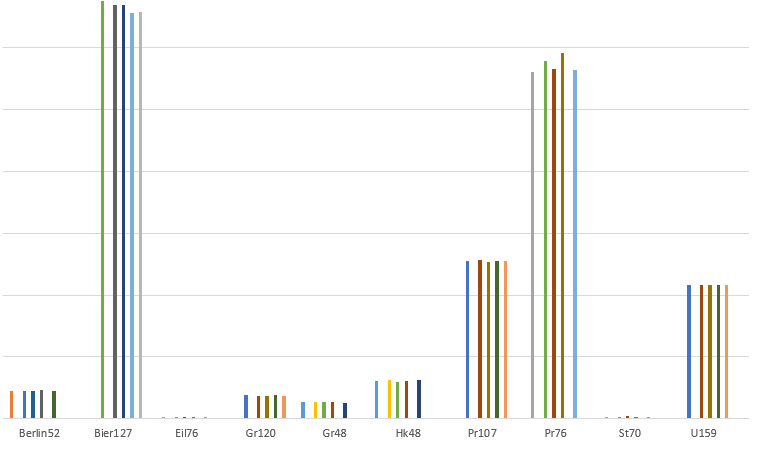
\includegraphics[scale=0.5]{test4photo3.png}
    \centering
    \caption{zależność funkcji kosztu od rozmiaru tablicy tabu dla podanych instancji}
  \end{figure}
  \subsection{Wnioski: }
  W wykonanych testach zauważyliśmy brak większych zalezności między długością listy tabu a otrzymanymi wynikami. 
  Brak klarownych rezultatów może być związany z niewielkimi rozmiarami, dla których były wykonywane testy, bądź z niewystarczającą
  liczbą iteracji algorytmu tabu.
  
